\chapter{경로적분에서 전파자와 꼭짓점까지}

입자와 그 상호작용을 살펴보기 전에, 핵심적인 구성이 무엇인지 분명히 해 두는 것이 좋다. 라그랑지안은 고전 장 방정식만 담는 것이 아니다. 경로적분을 통해 입자가 전파되고, 분열하고, 합쳐지고, 산란하는 진폭도 제공한다. 이것이 양자장론에서 파인만 도표로 가는 가장 직접적인 길이다.

\section{입자와 장의 최소 작용 원리}

파인만의 경로적분은 최소 작용 원리에 대응하는 양자역학적 구성이다. 좌표와 속도에 의존하는 라그랑지안을 갖는 보통의 뉴턴 입자에서 시작하자.\begin{equation}
\mathcal{L}=\mathcal{L}(x,\dot{x}),
\end{equation}어떤 궤적에 부여되는 작용은 다음과 같다.\begin{equation}
S[x]=\int \mathcal{L}(x,\dot{x})\,dt.
\end{equation}한 시공간 점에서 다른 점으로 가는 모든 후보 궤적에는 작용이 부여된다. 뉴턴 방정식을 만족하는지는 상관없다. 고전 궤적은 작용이 정지값을 갖는다는 점에서 구별된다. 전통적인 ``최소 작용''이라는 표현에서는 작용을 최소화한다고 말하지만, 정지값이라는 표현이 더 일반적이다. 정지 조건에서 고전 미분 운동 방정식이 나온다.

\begin{figure}[htbp]
\centering
\includegraphics[width=0.72\textwidth]{lecture_10_figure_02.png}
\caption{입자 궤적의 작용 적분.}
\lectureframe{00:02:14}
\end{figure}

고전 장에도 같은 구조가 적용된다. 모든 장을 일반적으로 \(\phi\)라고 쓰자. 국소적인 장 라그랑지안 밀도는 장과 그 공간 및 시간 미분 모두에 의존할 수 있다.\begin{equation}
\mathcal{L}
=\mathcal{L}\!\left(\phi,\frac{\partial\phi}{\partial x^\mu}\right)
=\mathcal{L}(\phi,\partial_\mu\phi).
\end{equation}상대론에 따르면 \(\mathcal{L}\)은 로런츠 스칼라로 변환해야 한다. 이 조건을 만족하는 한, 장과 그 미분으로 만든 스칼라 조합이 라그랑지안에 들어갈 수 있는 항을 이룬다.

\begin{figure}[htbp]
\centering
\includegraphics[width=0.62\textwidth]{lecture_10_figure_03.png}
\caption{장과 그 시공간 미분에 대한 장 라그랑지안의 의존성.}
\lectureframe{00:04:09}
\end{figure}

장의 경우 작용은 시공간 영역에 걸쳐 적분된다.\begin{equation}
S[\phi]=\int_{\Omega} d^4x\,\mathcal{L}(\phi,\partial_\mu\phi),
\qquad
d^4x=dt\,dx\,dy\,dz.
\end{equation}입자의 작용은 궤적을 따라 시간에 대해 적분한다. 장의 작용은 시공간 영역 전체에서 라그랑지안 밀도를 적분한 것이다.

입자 궤적의 양 끝점을 고정하는 것에 대응하는 조건은 초기 시간 단면과 최종 시간 단면에서 장의 전체 배치를 지정하는 것이다. 초기 장이 \(\phi_{\mathrm{i}}(\mathbf{x})\)이고 최종 장이 \(\phi_{\mathrm{f}}(\mathbf{x})\)라면, 그 사이의 시공간 전체를 보간하는 장이 놓인다. 경계 자료가 고전적인 보간 해를 허용하면, 경계 배치를 고정한 상태에서 그 해는 작용의 정지점이다.
\editorialnote{두 시간 단면에서 임의로 정한 장의 전체 배치가 반드시 고전 해를 허용하는 것은 아니다. 따라서 정지 작용에 관한 설명은 보간 해가 존재하는 경계 자료에 한정된다.}

기하학적으로 보면 장 이론에서 입자 궤적에 대응하는 것은 장의 이력이다.\footnote{시공간 영역은 대략 00:04:29의 도표를 바탕으로 재구성했다.}
\begin{figure}[htbp]
\centering
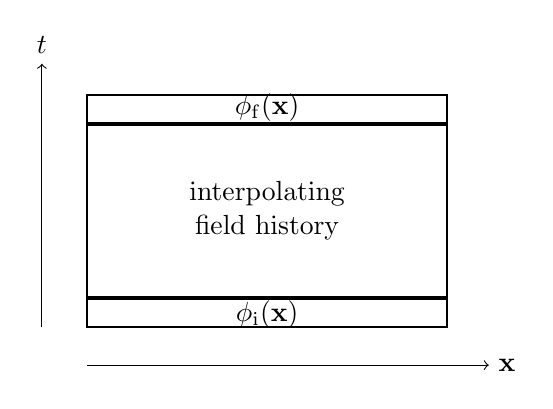
\begin{tikzpicture}[scale=0.88]
\draw[->] (-0.65,0) -- (-0.65,3.8) node[above] {$t$};
\draw[->] (0,-0.55) -- (5.8,-0.55) node[right] {$\mathbf{x}$};
\draw[thick] (0,0) rectangle (5.2,3.35);
\draw[very thick] (0,0.42) -- (5.2,0.42);
\draw[very thick] (0,2.93) -- (5.2,2.93);
\node at (2.6,0.18) {$\phi_{\mathrm{i}}(\mathbf{x})$};
\node at (2.6,3.17) {$\phi_{\mathrm{f}}(\mathbf{x})$};
\node[align=center] at (2.6,1.68) {interpolating\\field history};
\end{tikzpicture}
\caption{시공간 영역의 경계를 이루는 초기 및 최종 장 배치.}
\end{figure}

\begin{classroomqa}
\lecturetimestamp{00:07:34}
\audiencequestion{장이 이전과 같은 값으로 돌아올 수 있나요?}
\lecturerresponse{그렇습니다. 입자의 좌표가 이전 위치로 돌아오는 데 장애가 없듯이, 장이 이전 값으로 돌아오는 데도 아무런 장애가 없습니다.}
\end{classroomqa}

\begin{classroomqa}
\lecturetimestamp{00:07:46}
\audiencequestion{경계 자료가 장의 값인데 왜 시공간 사건이나 궤적을 말하나요?}
\lecturerresponse{입자 궤적은 장의 이력으로 바뀐다. 장 공간에서 각 끝점은 선택한 시간 단면에 놓인 장 전체를 뜻하며, 이력은 두 단면 사이의 시공간 영역에서 모든 점의 장을 지정한다.}
\end{classroomqa}

보간하는 장에 정지 작용 조건을 부과하면 편미분 방정식이 나온다. 장과 라그랑지안에 따라, 여기에는 맥스웰 방정식이나 중력 작용에서 나오는 아인슈타인 방정식 같은 식이 포함된다. 여기서는 변분을 자세히 유도할 필요가 없다. 중요한 흐름은 다음과 같다.\begin{equation}
\mathcal{L}
\longrightarrow
S[\phi]
\longrightarrow
\text{classical field equations}.
\end{equation}

\section{파인만의 입자 경로 합}

양자역학에서는 어떤 궤적이 실제로 일어나는지를 묻는 대신 진폭을 묻는다. \((x,t)\)에서 입자를 넣고, 잠시 눈을 감았다가, \((x',t')\)에서 검출기를 켠다고 생각해 보자. 진폭은 다음과 같다.\begin{equation}
\mathcal{A}(x,t;x',t')
\end{equation}이는 복소수다. 그 절댓값의 제곱이 확률이다.\begin{equation}
\begin{aligned}
P(x,t;x',t')
&=\left|\mathcal{A}(x,t;x',t')\right|^2\\
&=\mathcal{A}(x,t;x',t')
\mathcal{A}(x,t;x',t')^*.
\end{aligned}
\end{equation}

파인만의 규칙은 모든 후보 경로에 작용을 부여하고, 각 경로에 다음 위상을 대응시킨다.\begin{equation}
\exp\!\left(-\frac{i}{\hbar}S[x]\right)
=
\exp\!\left[-\frac{i}{\hbar}\int \mathcal{L}(x,\dot{x})\,dt\right].
\end{equation}

\begin{figure}[htbp]
\centering
\includegraphics[width=0.70\textwidth]{lecture_10_figure_04.png}
\caption{입자 경로에 대응하는 복소 위상.}
\lectureframe{00:11:52}
\end{figure}

지수의 차원을 없애려면 \(\hbar\) 인자가 필요하다.\footnote{00:11:52에 칠판에 적힌 식은 \(e^{-i\int\mathcal{L}\,dt}\)로 읽으면 자연스럽다. \(\hbar\) 인자는 00:12:02에 말로 덧붙여진다.}전이 진폭은 양 끝점을 잇는 가능한 모든 경로의 위상을 합한 것이다.\begin{equation}
\mathcal{A}(x,t;x',t')
=
\sum_{\substack{\text{paths }x(\tau)\\(x,t)\rightarrow(x',t')}}
\exp\!\left(-\frac{i}{\hbar}S[x]\right).
\end{equation}여기서 ``가능한 경로''란 뉴턴 방정식의 해를 뜻하지 않는다. 합에 포함되는 임의의 경로를 뜻한다. 비상대론적 양자역학에서 경로는 시간을 거슬러 되돌아가지 않고 앞으로 나아간다. 플랑크 상수의 차원은 작용이므로 \(S/\hbar\)은 무차원이다.

연속하는 작은 단계들의 진폭이 곱해지므로 지수함수가 자연스럽게 나타난다. 경로를 연이어 이어지는 여러 구간으로 나누면 작용은 더해진다.\begin{equation}
S=S_1+S_2+\cdots,
\end{equation}반면 위상은 곱해진다.\begin{equation}
e^{-iS/\hbar}
=e^{-iS_1/\hbar}e^{-iS_2/\hbar}\cdots.
\end{equation}인자 \(i\)는 단순한 장부상의 표기가 아니라 양자역학 규칙의 일부다.

\begin{classroomqa}
\lecturetimestamp{00:13:27}
\audiencequestion{지수함수는 연속하는 작은 단계들의 진폭을 곱하는 것과 관련이 있나요?}
\lecturerresponse{그렇습니다. 연속하는 단계들의 진폭은 곱해지고, 이에 대응하는 작용의 각 구간은 더해집니다.}
\end{classroomqa}

\begin{classroomqa}
\lecturetimestamp{00:13:49}
\audiencequestion{경로의 합 자체가 확률인가요?}
\lecturerresponse{아닙니다. 경로의 합은 일반적으로 복소수인 확률 진폭이다. 여기에 복소켤레를 곱하면 확률이 나온다.}
\end{classroomqa}

\section{장 이력에 대한 합}

같은 정식화는 양자장론에도 확장되지만, 여기서의 구성은 의도적으로 엄밀성을 추구하지 않는다. 초기 장 배치 \(\phi(\mathbf{x})\)와 별도로 지정한 최종 장 배치 \(\phi'(\mathbf{x})\)에서 시작하자. 이는 고립된 두 점의 값이 아니라 공간 전체에서 정의된 함수다.

공간의 모든 점에서 장을 준비하고, 계를 시간에 따라 진화시킨 뒤, 나중에 모든 점에서 장을 측정하는 이상화된 장치를 생각해 볼 수 있다. 그런 장치는 현실적이지 않지만, 개념적인 질문을 명확히 해 준다. 초기의 장 전체 배치에서 최종 배치로 가는 진폭은 얼마인가?

상상할 수 있는 모든 보간 장 이력이 기여한다. 각 이력에 대해 다음을 계산하고,\begin{equation}
S[\phi]=\int d^4x\,\mathcal{L}(\phi,\partial_\mu\phi)
\end{equation}이에 대응하는 위상을 붙인다. 개략적으로 쓰면 다음과 같다.\begin{equation}
\mathcal{A}\!\left[\phi(\mathbf{x})\rightarrow\phi'(\mathbf{x})\right]
=
\sum_{\substack{\text{field histories}\\
\phi_{\mathrm{i}}=\phi,\;\phi_{\mathrm{f}}=\phi'}}
\exp\!\left(-\frac{i}{\hbar}S[\phi]\right).
\end{equation}이력은 고전 장 방정식을 풀 필요가 없다. 그저 사이에 놓인 시공간 영역 전체에서 장의 값을 완전히 지정한 하나의 배치다.

\begin{classroomqa}
\lecturetimestamp{00:17:39}
\audiencequestion{가능한 경로는 무한히 많고, 각 위상의 크기는 1입니다. 그런데 어떻게 그 합이 수렴할 수 있나요? 경로들을 최소화하는 건가요?}
\lecturerresponse{경로들을 합하는 것이지 최소화하는 것이 아닙니다. 각 항은 단위원 위에 분포한 위상이므로 서로 상쇄될 수 있습니다. 이는 영보다 일정한 양만큼 큰 항들을 무한히 더하는 경우와 다릅니다. 진동 적분은 수렴할 수 있으며, 델타 함수의 푸리에 표현이 익숙한 예입니다. 위상들이 원 위에 균일하게 분포한다면 그 벡터 합은 0이 됩니다. 대부분의 경로는 강하게 상쇄됩니다. 위상이 가장 느리게 변하는 까닭에 작용이 정지하는 경로 근처의 경로들은 상쇄가 가장 적게 일어나며, 이로써 고전적 극한이 나타납니다.}
\end{classroomqa}

\editorialnote{실시간 경로적분에는 보통 수렴 처방이 필요하다. 여기서 단위원을 이용한 논의는 진동에 따른 상쇄 논증을 설명할 뿐, 일반적인 수렴 증명을 제시하는 것은 아니다.}

이 상쇄를 복소평면에서의 벡터 합으로 그려 볼 수 있다.\footnote{단위원 구성은 00:18:32--00:20:21의 칠판 설명을 바탕으로 재구성했다.}
\begin{figure}[htbp]
\centering
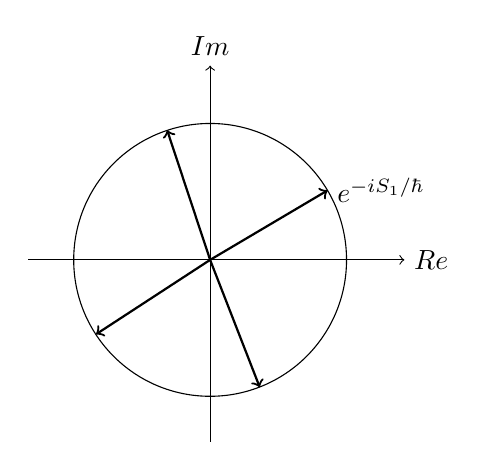
\begin{tikzpicture}[scale=1.05]
\draw[->] (-2.2,0) -- (2.35,0) node[right] {$\operatorname{Re}$};
\draw[->] (0,-2.2) -- (0,2.35) node[above] {$\operatorname{Im}$};
\draw (0,0) circle (1.65);
\draw[thick,->] (0,0) -- (1.42,0.84);
\draw[thick,->] (0,0) -- (-1.38,-0.90);
\draw[thick,->] (0,0) -- (-0.52,1.57);
\draw[thick,->] (0,0) -- (0.60,-1.54);
\node[right] at (1.42,0.84) {$e^{-iS_1/\hbar}$};
\end{tikzpicture}
\caption{방향이 서로 다른 단위 크기의 위상들은 상쇄될 수 있다.}
\end{figure}

실제로,\begin{equation}
e^{-iS/\hbar}
=
\cos\!\left(\frac{S}{\hbar}\right)
-i\sin\!\left(\frac{S}{\hbar}\right).
\end{equation}각 기여는 단위 벡터다. 방향이 다른 기여들은 더해질 뿐 아니라 서로 빼기도 한다. \(S\)의 정지점 근처에서는 인접한 이력들의 위상이 거의 같으므로, 그 기여들이 더 효과적으로 서로 보강된다. 정지 작용에서 멀어지면 위상이 빠르게 변하고, 파괴 간섭이 우세해진다.

이 경로적분 구조는 사실상 모든 현대 양자장론의 바탕이다. 다음에 다룰 실용적인 단계는 유도하지 않고 서술하겠다. 계산으로 들어가는 다소 지나치게 단순화된 방법이지만, 같은 대상을 두 가지 언어로 어떻게 다루는지 보여 준다.

어떤 과정을 계산한다는 것은 초기에서 최종 상태로의 전이 확률을 계산한다는 뜻이다. 한 가지 설명에서는 초기 장 배치와 최종 장 배치를 지정한다. 다른 설명에서는 들어오는 입자와 나가는 입자, 즉 하나 이상의 장에 속하는 양자를 지정한다. 이 질문들은 서로 달라 보이지만, 둘 다 같은 장 이론의 경로적분으로 계산한다.

\section{이산 시공간 형식}

장 이력의 합에 구체적인 의미를 부여하기 위해 시공간을 작은 셀들로 나누고 각 셀에 장의 값을 하나씩 지정하자. 셀의 크기를 줄이면 연속체 극한에 가까워지지만, 지금은 셀을 유한한 크기로 둔다. 이렇게 하면 함수에 대한 형식적인 합이 격자 셀에 수를 배정하는 경우들의 합으로 바뀐다.

앞서 살펴본 직관적인 방법에서는 각 셀마다 \(1+\mathcal{L}_i\)과 비슷한 인자의 곱을 사용한 다음, 입자의 전파와 충돌을 나타내는 항을 식별한다. 이 구성은 매우 중요하므로 다시 살펴볼 만하지만, 인자를 바로잡아야 한다. 작은 양은 라그랑지안 자체가 아니다. 셀 안에 포함된 작용이다.

셀의 시공간 부피가 다음과 같다면\begin{equation}
a^4=\Delta t\,\Delta x\,\Delta y\,\Delta z,
\end{equation}그 작용은 다음과 같다.\begin{equation}
A_i=\mathcal{L}_i a^4.
\end{equation}\(A_i\)는 셀이 작으므로 작다. 잠시 \(\hbar\)를 생략하면, 바로잡은 기본 인자는\begin{equation}
1-iA_i,
\end{equation}이며, \(1+\mathcal{L}_i\)가 아니다.

임의의 작은 \(\epsilon\)에 대해,\begin{equation}
1+\epsilon\simeq e^\epsilon,
\end{equation}이다. 왜냐하면\begin{equation}
e^\epsilon
=1+\epsilon+\frac{\epsilon^2}{2!}
+\frac{\epsilon^3}{3!}+\cdots.
\end{equation}이기 때문이다. 따라서 이 임시 단위계에서는 셀이 충분히 작을 때 \(1-iA_i\)이 \(e^{-iA_i}\)를 근사한다. 처음부터 정확한 지수 인자를 사용하는 편이 더 깔끔하다.

\begin{classroomqa}
\lecturetimestamp{00:27:57}
\audiencequestion{지수함수에 \(\hbar\) 인자가 필요한가요?}
\lecturerresponse{그렇습니다. 무차원인 셀 인자는 1차까지 \(1-iA_i/\hbar\)이고, 정확한 지수함수는 \(\exp(-iA_i/\hbar)\)이다. 나중에 \(\hbar=1\)인 단위계를 택할 수 있다.}
\end{classroomqa}

\(\hbar\)를 다시 포함하면, 수정된 중간 인자와 그 지수형은 다음과 같다.\begin{equation}
1-\frac{i}{\hbar}A_i
\simeq
\exp\!\left(-\frac{i}{\hbar}A_i\right).
\end{equation}

하나의 고정된 이력에 대해 시공간 적분을 셀 작용들의 합으로 바꾸면 다음과 같다.\begin{equation}
S[\phi]
=\int d^4x\,\mathcal{L}
\;\longrightarrow\;
\sum_i A_i.
\end{equation}그 이력의 위상은 다음과 같다.\begin{equation}
\exp\!\left(-\frac{i}{\hbar}\sum_i A_i\right).
\end{equation}합의 지수함수는 지수함수들의 곱이다.\begin{equation}
\exp\!\left(-\frac{i}{\hbar}\sum_i A_i\right)
=
\prod_i\exp\!\left(-\frac{i}{\hbar}A_i\right).
\end{equation}연산 순서가 중요하다. 먼저 하나의 완전한 이력을 고르고 그 셀 가중치들을 곱한다. 그런 다음에야 서로 다른 이력들을 합산한다.

격자를 사용하면 경계 자료도 명시적으로 드러난다.\footnote{체커보드와 고정된 첫째 행 및 마지막 행은 대략 00:23:54 및 00:30:49의 도표를 바탕으로 재구성했다.}
\begin{figure}[htbp]
\centering
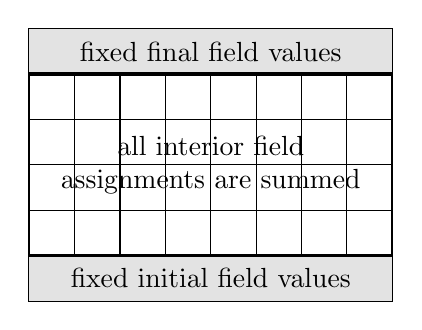
\begin{tikzpicture}[scale=0.72]
\draw[step=0.8,thin] (0,0) grid (6.4,4.8);
\draw[thick] (0,0) rectangle (6.4,4.8);
\fill[gray!22] (0,0) rectangle (6.4,0.8);
\fill[gray!22] (0,4.0) rectangle (6.4,4.8);
\draw[very thick] (0,0.8) -- (6.4,0.8);
\draw[very thick] (0,4.0) -- (6.4,4.0);
\node at (3.2,0.4) {fixed initial field values};
\node at (3.2,4.4) {fixed final field values};
\node[align=center] at (3.2,2.4) {all interior field\\assignments are summed};
\end{tikzpicture}
\caption{초기 및 최종 격자 행을 고정한 이산 장 이력.}
\end{figure}

첫째 행은 초기 장 배치를 지정하고, 마지막 행은 최종 배치를 지정한다. 내부 셀마다 이산화에 포함된 모든 장 값을 허용한다. 따라서 전이 진폭은 다음과 같은 개략적인 형태를 갖는다.\begin{equation}
\mathcal{A}\!\left[\phi_{\mathrm{i}}\rightarrow\phi_{\mathrm{f}}\right]
=
\sum_{\{\phi\}_{\mathrm{interior}}}
\prod_i\exp\!\left(-\frac{i}{\hbar}A_i[\phi]\right),
\end{equation}첫째 행과 마지막 행은 고정한다. 바꾸어 말하면, 각 내부 배치에 대해 전체 작용의 지수함수를 계산한 뒤, 그 기여를 다른 모든 배치의 기여에 더한다.

\section{장 배치에서 입자 배치까지}

같은 전이 진폭을 장의 관점이나 입자의 관점에서 설명할 수 있다. 첫째와 마지막 시간 단면에서 장을 고정하는 대신, 들어오는 장 양자와 나가는 장 양자의 모임을 지정하고 그 둘을 연결하는 진폭을 물을 수 있다. 계산하는 대상은 같다. 달라진 것은 경계를 기술하는 방식뿐이다.

양자장에는 생성 연산자와 소멸 연산자가 들어 있다. 따라서 장의 곱은 입자 상태에 작용하여 양자를 생성하거나 소멸시키거나 이동시킨다. 이러한 연산자 해석을 통해 격자 경로적분은 입자 규칙들의 집합으로 바뀐다.

\begin{classroomqa}
\lecturetimestamp{00:34:11}
\audiencequestion{장 양자는 반드시 입자로 식별될 수 있나요?}
\lecturerresponse{전통적인 의미에서 개별적으로 관측 가능한 입자로 항상 식별되는 것은 아니다. 예를 들어 쿼크는 쿼크장의 양자이지만, 가둠 때문에 고립된 쿼크가 빠져나와 단독으로 검출될 수 없다. 더 일반적으로, 이론에서 이름 붙인 장과 통상적으로 관측 가능한 입자 종 사이에 일대일 대응이 성립할 필요는 없다. 그런 단순한 대응 관계를 허용하지 않는 장 이론도 있다. ``입자''를 에너지와 다른 양자수를 지닌 불가분의 양자라는 넓은 의미로 사용한다면, 그 구분은 부분적으로 용어상의 차이가 될 수 있다.}
\end{classroomqa}

\editorialnote{00:35:45--00:36:08에서 원문이 언급한 약결합 조건절은 문법적으로 모호하여 여기서는 해석을 확정하지 않았다. 확실하게 말할 수 있는 내용은 장의 명칭과 통상적으로 관측 가능한 입자 종이 일대일로 대응할 필요는 없다는 것이다.}

격자 합은 여전히 장의 값 전체를 범위로 한다. 고전적인 매끄러운 해와 비슷한 배치로 제한되지 않는다.

\begin{classroomqa}
\lecturetimestamp{00:36:44}
\audiencequestion{장 이력은 연속적이거나 적어도 대략 연속적이어야 하나요?}
\lecturerresponse{아니다. 이산 격자에서는 이웃한 셀마다 장의 값이 놓일 뿐이며, 모든 배치를 합에 포함한다. 대략 연속적인 이력으로 제한하지 않는다. 양자장은 크게 요동하므로, 전형적인 이력은 매끄러운 고전장이 아니다.}
\end{classroomqa}

독립적으로 지정하는 변수는 격자점 또는 격자 셀에서의 장 값이다. 미분은 이웃한 값들의 차이로 구한다.

\begin{classroomqa}
\lecturetimestamp{00:37:56}
\audiencequestion{장과 그 미분의 값을 각각 독립적으로 지정하나요?}
\lecturerresponse{아니다. 장의 값은 격자점에 지정한다. 미분은 이웃한 장 값들의 차이로 재구성한다. 유한차분을 정의하는 방법은 여러 가지지만, 미분은 추가적인 독립 변수가 아니다.}
\end{classroomqa}

따라서 격자 간격 \(a\)에 대해 개략적으로 다음과 같이 쓸 수 있다.\begin{equation}
\partial_\mu\phi(x)
\longrightarrow
\frac{\phi(x+a\hat\mu)-\phi(x)}{a}.
\end{equation}장 값의 축도 작은 구간들로 나눌 수 있으며, 그러면 각 격자점에서 가능한 값들의 집합은 셀 수 있게 된다.

\begin{classroomqa}
\lecturetimestamp{00:38:53}
\audiencequestion{장이 둘 이상이면 무엇이 달라지나요?}
\lecturerresponse{각 격자점에서 각 장의 값을 하나씩 지정하고, 그 모든 배치를 합산한다.}
\end{classroomqa}

복소수 값을 갖는 장을 복소 변수의 해석함수와 혼동해서는 안 된다. 해석성은 매우 강한 매끄러움 조건이다. 장 경로적분에 들어가는 이력은 그 조건을 따를 필요가 없으며, 일반적으로 대략 매끄럽기조차 하지 않다.

\begin{classroomqa}
\lecturetimestamp{00:39:07}
\audiencequestion{장이 복소수 값을 가지면 해석함수가 만족하는 매끄러움 조건도 만족해야 하나요?}
\lecturerresponse{아니다. 복소수 값을 갖는다는 것이 해석적이라는 뜻은 아니다. 해석함수 이론은 매우 매끄럽고 엄격한 제약을 받는 함수 부류를 다룬다. 여기서 합산하는 장 이력은 위치의 해석함수일 필요가 없다. 전형적인 이력은 매우 불규칙하며, 연속체 극한에서는 매우 불연속적이라고 볼 수 있다.}
\end{classroomqa}

이렇게 얻은 계산은 벅차 보인다. 시공간과 장 값을 모두 이산화한 뒤에도 표본으로 삼아야 할 배치가 엄청나게 많을 수 있다.

\begin{classroomqa}
\lecturetimestamp{00:40:04}
\audiencequestion{컴퓨터는 표본으로 삼을 격자 배치의 수를 어떻게 알며, 계산이 언제 수렴했는지는 어떻게 판단하나요?}
\lecturerresponse{그 질문은 격자 게이지 이론, 또는 더 일반적으로 격자 양자장론의 주제다. 이제는 효과적으로 계산을 수행하는 분야가 되었다. 나는 격자 게이지 이론의 규칙을 처음 세우는 데 참여했지만, 이후의 컴퓨터 기술 개발에는 관여하지 않았다. 규칙을 세우는 데는 약 3주가 걸렸고, 이런 계산을 수행할 기술을 개발하는 데는 30년쯤 걸렸다. 실제적인 지식의 상당 부분은 통계역학에서 얻었다. 통계역학에서도 격자 배치들에 대한 합으로 분배함수를 구한다---예컨대 결정의 각 격자점이 차 있는지를 합산한다. 충분한 배치를 표본으로 삼았는지 판단하는 것은 기술적인 문제다. 전문가들은 계산이 통제되고 있는 때를 안다---고 생각한다---그리고 그렇게 얻은 계산 결과는 실험과 일치한다.}
\end{classroomqa}

격자 게이지 이론의 개념적 규칙은 빠르게 마련됐지만, 그 규칙으로 계산하는 데 필요한 기술은 훨씬 오랜 시간이 걸려 개발됐다. 체커보드는 단순한 비유가 아니다. 실제 계산 방법의 출발점이기도 하다.

\section{이차항과 입자 전파}

이제 장의 연산자 해석으로 돌아가자. 이웃한 두 격자점 \(x\)와 \(x'\)에 대해 곱은\begin{equation}
\phi(x)\phi(x')
\end{equation}적절한 단일 입자 행렬원소에서 한 격자점의 입자를 소멸시키고 다른 격자점에 입자를 생성하는 일을 할 수 있다. 따라서 해당 입자 부문에서는 한 링크를 따라 이동하는 것으로 그려 볼 수 있다. 이는 연산자 곱을 해석하는 한 가지 방법일 뿐, 유일한 해석은 아니다.

이런 링크를 만들어 내는 항은 미분항이다. 엄밀히 말해 이 항은 하나의 셀이 아니라 이웃한 두 셀의 쌍과 관련된다. 예를 들어 시간 미분은 다음과 같이 바뀐다.\begin{equation}
\partial_t\phi(t,\mathbf{x})
\longrightarrow
\frac{\phi(t+a,\mathbf{x})-\phi(t,\mathbf{x})}{a},
\end{equation}공간 미분도 공간 링크를 따라 같은 방식으로 다룬다.

\begin{classroomqa}
\lecturetimestamp{00:44:39}
\audiencequestion{여기서 다루는 라그랑지안에 이차 미분이 포함되나요?}
\lecturerresponse{여기서 고려하는 표준 이론은 일차 미분을 사용해 표현한다. 따라서 격자 이론에서는 이웃한 격자점 사이의 일차 차분을 사용한다.}
\end{classroomqa}

일차 차분을 제곱하면 같은 격자점에 대한 항과 이웃한 격자점 사이의 교차항이 모두 생긴다.\begin{align}
\frac{1}{2}\bigl[\phi(x)-\phi(x')\bigr]^2
&=
\frac{1}{2}\phi(x)^2
+\frac{1}{2}\phi(x')^2
-\phi(x)\phi(x').
\end{align}교차항은 한 격자점에서 다른 격자점으로의 이동을 나타낼 수 있다. 두 제곱항은 각각 같은 격자점에 대한 항이다. 이차 미분항은 운동항이며, 전파를 구성할 때 먼저 사용할 것은 그중 이웃한 격자점 사이의 교차항이다.

조합 구조를 분리해 보기 위해 이웃한 격자점 곱들을 모아 다음과 같이 두자.\begin{equation}
K=\sum_{\langle x,x'\rangle}\phi(x)\phi(x').
\end{equation}경로적분 가중치의 해당 인자는 개략적으로 다음과 같이 쓴다.\begin{equation}
e^{-iK}.
\end{equation}\editorialnote{이 개략적인 격자 인자에서는 격자 간격의 거듭제곱, \(\hbar\), 계량 부호, 정규화 상수와 링크 계수를 생략했다.}이를 전개하면\begin{equation}
e^{-iK}
=1-iK-\frac{1}{2!}K^2+\frac{i}{3!}K^3+\cdots,
\end{equation}또는 이웃 격자점에 대한 합을 드러내어 쓰면 다음과 같다.\begin{align}
e^{-iK}
={}&1
-i\sum_{\langle x,x'\rangle}\phi(x)\phi(x')
\nonumber\\
&-\frac{1}{2!}
\sum_{\langle x,x'\rangle}
\sum_{\langle y,y'\rangle}
\phi(x)\phi(x')\phi(y)\phi(y')
+\cdots .
\end{align}각 인자는 이웃한 격자점 쌍 하나를 독립적으로 선택한다.

입자 도표에는 매달린 끝이 없어야 한다. 드러난 끝점은 초기 단면에서 입자를 넣거나 최종 단면에서 입자를 제거한다고 경계 조건에 명시된 경우에만 허용된다. 내부에 고립된 링크는 끝이 짝을 이루지 않으므로, 지정된 전이에 대한 완전한 기여를 나타내지 않는다. 내부 링크의 끝들은 서로 이어져야 한다.

시간층이 두 개뿐인 격자를 먼저 생각해 보자. 초기 상태에서 \(x\)에 입자를 넣고 최종 상태에서 이웃 점 \(x'\)에서 입자를 제거하면, 1차 항이 두 경계 삽입을 연결할 수 있다.\begin{equation}
x\longrightarrow x',
\qquad
\mathcal{A}_{\text{one link}}\sim -i.
\end{equation}계수 \(-i\)는 이 개략적 전개에서의 계수일 뿐이며, 생략한 격자 및 정규화 인자는 그대로 고려해야 한다.

\begin{classroomqa}
\lecturetimestamp{00:52:16}
\audiencequestion{1차 한 링크 항은 관련된 초기 격자점과 최종 격자점이 서로 이웃할 때만 기여하나요?}
\lecturerresponse{그렇다. 그 항은 이웃한 격자점 쌍 하나를 선택하므로, 경계의 두 격자점이 서로 이웃할 때만 연결할 수 있다. 더 멀리 전파되는 경우는 고차 곱에서 나온다.}
\end{classroomqa}

2차에서는 두 인자가 각각 이웃한 격자점 쌍에 대해 독립적으로 합산된다.\begin{equation}
K^2
=
\sum_{\langle x,x'\rangle}
\sum_{\langle y,y'\rangle}
\phi(x)\phi(x')\phi(y)\phi(y').
\end{equation}

\begin{classroomqa}
\lecturetimestamp{00:52:40}
\audiencequestion{두 번째 이웃 격자점 쌍은 첫 번째 인자가 고른 쌍과 이어져야 하나요?}
\lecturerresponse{아니다. 각 인자는 이웃한 격자점 쌍을 독립적으로 선택한다. 두 쌍은 한 격자점을 공유할 수도, 완전히 떨어져 있을 수도, 심지어 같은 쌍일 수도 있다. 합에는 모든 경우가 포함된다.}
\end{classroomqa}

세 시간층에 걸쳐 전파되는 입자 하나에 유용한 2차 선택은 중간 격자점을 공유한다.\begin{equation}
\bigl[\phi(x_0)\phi(x_1)\bigr]
\bigl[\phi(x_1)\phi(x_2)\bigr],
\qquad
x_0\longrightarrow x_1\longrightarrow x_2.
\end{equation}첫 번째 링크의 끝은 두 번째 링크의 시작과 이어진다. \(x_0\)의 초기 끝점과 \(x_2\)의 최종 끝점만 드러나 있으므로, 이 항은 필요한 단일 입자 전이에 기여한다. 개략적인 지수 전개에서 그 계수는 다음과 같다.\begin{equation}
-\frac{1}{2!}.
\end{equation}

선택된 링크들이 서로 떨어진 홉을 이룰 수도 있다.\footnote{링크 도표는 00:49:18--00:55:12에 나온 순서를 바탕으로 재구성했다.}
\begin{figure}[htbp]
\centering
\resizebox{\linewidth}{!}{%
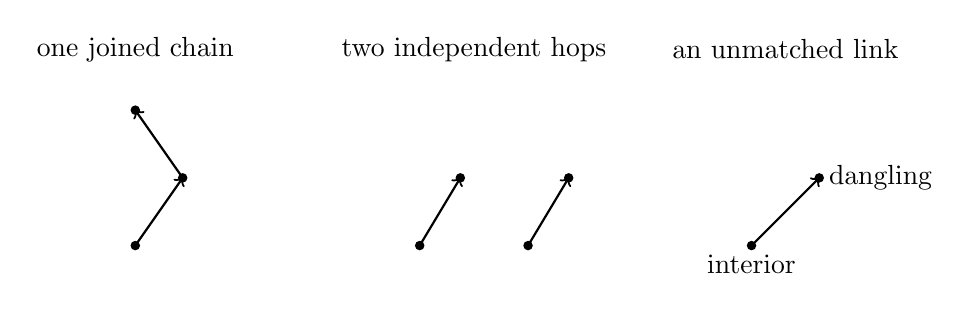
\begin{tikzpicture}[scale=0.86]
\node at (0,2.9) {one joined chain};
\fill (0,0) circle (2pt);
\fill (0.7,1.0) circle (2pt);
\fill (0,2.0) circle (2pt);
\draw[thick,->] (0,0) -- (0.7,1.0);
\draw[thick,->] (0.7,1.0) -- (0,2.0);

\begin{scope}[xshift=4.2cm]
\node at (0.8,2.9) {two independent hops};
\fill (0,0) circle (2pt);
\fill (0.6,1.0) circle (2pt);
\fill (1.6,0) circle (2pt);
\fill (2.2,1.0) circle (2pt);
\draw[thick,->] (0,0) -- (0.6,1.0);
\draw[thick,->] (1.6,0) -- (2.2,1.0);
\end{scope}

\begin{scope}[xshift=9.1cm]
\node at (0.5,2.9) {an unmatched link};
\fill (0,0) circle (2pt);
\fill (1.0,1.0) circle (2pt);
\draw[thick,->] (0,0) -- (1.0,1.0);
\node[below] at (0,0) {interior};
\node[right] at (1.0,1.0) {dangling};
\end{scope}
\end{tikzpicture}%
}
\caption{서로 이어진 링크 선택, 독립적인 링크 선택, 그리고 끝이 짝을 이루지 않는 링크 선택.}
\end{figure}

이 차수에서도 이미 경로가 둘 이상일 수 있다. 시간 방향으로 한 격자 간격, 공간 방향으로 한 격자 간격만큼 변위할 때 다음 두 순서는\begin{align}
x
&\longrightarrow x+\hat t
\longrightarrow x+\hat t+\hat s,\\
x
&\longrightarrow x+\hat s
\longrightarrow x+\hat s+\hat t
\end{align}같은 끝점에 도달한다.

\begin{classroomqa}
\lecturetimestamp{00:55:53}
\audiencequestion{같은 대각선 끝점에 도달하는 두 단계 경로가 또 있나요?}
\lecturerresponse{그렇다. 시간 방향으로 먼저 이동하고 공간 방향으로 나중에 이동할 수도 있고, 순서를 바꾸어 이동할 수도 있다. 두 경로 모두 같은 전이 진폭에 기여한다.}
\end{classroomqa}

두 링크에서 멈출 이유는 없다. 3차 항은 이웃한 링크 세 개로 이어지는 사슬을 제공한다. 경로는 곧장 나아갈 수도, 우회할 수도, 최종점에 도달하기 전에 멀어졌다가 되돌아올 수도 있다. 더 높은 차수에는 더 긴 우회 경로와 반복적인 왕복 이동이 포함된다. 따라서 임의의 차수까지 전개하면 국소적인 링크들을 이어 만든 모든 경로가 기여한다. 한 점에서 다른 점으로 가는 진폭은 이 모든 경로의 합이며, 계수에는 \(i\)의 적절한 거듭제곱과 계승이 들어간다.\begin{equation}
\begin{gathered}
\mathcal{A}(x_{\mathrm{in}}\to x_{\mathrm{out}})
=
\sum_{\text{joined lattice routes }r}c_r,
\\
c_r\ \hbox{read from the exponential expansion}.
\end{gathered}
\end{equation}계수는 일반적으로 복소수이므로 결과 진폭도 복소수다.

상대론적 전파에서는 또 다른 가능성이 생긴다. 경로는 시간 방향으로 위쪽과 아래쪽 모두를 향할 수 있으며, 같은 링크를 여러 번 지날 수도 있다.

\begin{classroomqa}
\lecturetimestamp{00:58:47}
\audiencequestion{경로가 같은 두 셀을 계속해서 반복해 지날 수 있나요?}
\lecturerresponse{그렇다. 반복해서 지나는 경로도 포함되며, 상대론적 전개에서는 시간상 뒤로 진행할 수도 있다.}
\end{classroomqa}

시간을 거슬러 가는 구간은 서로 동등한 두 가지 방식으로 그림을 해석할 수 있다. 입자 선이 시간을 거슬러 달리는 것으로 볼 수 있다. 또는 시간은 앞으로만 흐른다고 보고 따라가면, 입자--반입자 쌍이 생성되고 입자 쪽은 앞으로 계속 진행하며, 반입자는 나중에 원래 입자와 만나 소멸한다. 두 설명은 같은 하나의 연결된 선에 담겨 있다.\footnote{두 가지 해석은 00:59:00--00:59:51의 도표와 설명에 따른다.}

\begin{figure}[htbp]
\centering
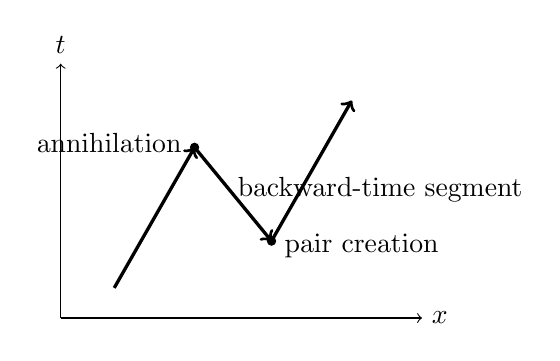
\begin{tikzpicture}[scale=0.85]
\draw[->] (0,0) -- (0,3.8) node[above] {$t$};
\draw[->] (0,0) -- (5.4,0) node[right] {$x$};
\draw[very thick,->] (0.8,0.45) -- (2.0,2.55);
\draw[very thick,->] (2.0,2.55) -- (3.15,1.15);
\draw[very thick,->] (3.15,1.15) -- (4.35,3.25);
\fill (2.0,2.55) circle (2pt);
\fill (3.15,1.15) circle (2pt);
\node[left] at (1.95,2.62) {annihilation};
\node[right] at (3.20,1.08) {pair creation};
\node[right] at (2.50,1.92) {backward-time segment};
\end{tikzpicture}
\caption{시간을 거슬러 가는 구간을 앞으로 진행하는 쌍생성과 소멸로 해석한 그림.}
\end{figure}

고차에서 나타나는 계승은 지수함수의 거듭제곱급수를 제어하지만, 이것이 장 배치 전체에 대한 합까지 제어한다는 뜻은 아니다.

\begin{classroomqa}
\lecturetimestamp{01:00:00}
\audiencequestion{\(1/n!\) 인자가 수렴을 보장하나요?}
\lecturerresponse{고정된 인수에 대해서는 지수급수의 수렴을 보장합니다. 그러나 이것만으로 장 배치 전체에 대한 별도의 합이 수렴한다고 보장할 수는 없습니다. 이는 서로 다른 문제입니다. 유한 격자에서 장의 값이 유한 개로 이산화되어 있으면 배치의 수는 유한하지만, 연속체 극한과 무한 부피 극한을 취하려면 추가적인 제어가 필요합니다.}
\end{classroomqa}

\section{하나의 링크 곱, 여러 입자 해석}

2차 곱에는 한 입자의 전파보다 더 많은 것이 담겨 있다. 이웃한 두 쌍이 한 끝점을 공유하면, 다음과 같은 두 링크 사슬을 따라 입자 하나를 이동시킬 수 있다.
\begin{equation}
\bigl[\phi(x_0)\phi(x_1)\bigr]
\bigl[\phi(x_1)\phi(x_2)\bigr].
\end{equation}
선택한 쌍들이 서로 떨어져 있으면, 같은 2차 항은 입자 두 개를 각각 한 링크씩 이동시킬 수 있다.\footnote{한 입자의 전파와 서로 독립적인 두 번의 한 링크 도약에 대한 비교는 01:00:46--01:02:34의 판서 내용을 바탕으로 재구성한 것이다.}
\begin{equation}
\bigl[\phi(x_0)\phi(x_1)\bigr]
\bigl[\phi(y_0)\phi(y_1)\bigr],
\qquad x_0\neq y_0.
\end{equation}
첫 번째 인자는 입자 하나를 전달하고 두 번째 인자는 다른 입자를 전달한다. 따라서 격자 전개의 2차 항에는 모든 다입자 부문에서의 전파 진폭이 들어 있다. 같은 대수적 차수라도 하나의 더 긴 연결 경로를 나타낼 수도 있고, 더 짧은 비연결 경로 여러 개를 나타낼 수도 있다.

여기에는 정보가 상당히 많이 담겨 있지만, 아직 진정한 상호작용 꼭짓점은 아니다. 이차 전파 항만으로는 연결된 입자 선의 수가 달라지도록 갈라지지 않는다. 국소 연산자 곱을 여러 생성 및 소멸 과정으로 해석할 수는 있지만, 입자 수가 변하는 과정에는 추가 상호작용이 필요하다.

\begin{classroomqa}
\lecturetimestamp{01:03:30}
\audiencequestion{전자와 양전자가 소멸하여 아무 입자도 남기지 않을 수 있을까요?}
\lecturerresponse{들어오는 에너지는 영이 아닌데 에너지를 운반하는 최종 상태가 없는 기여는 에너지 보존에 어긋납니다. 가능한 모든 시공간 위치에 대해 합하면 진폭들이 상쇄됩니다. 전자--양전자 소멸은 다른 장이 에너지를 가져갈 때 일어날 수 있습니다---예를 들어 전자기 양자가 생성될 때가 그렇습니다.}
\end{classroomqa}

\editorialnote{요약된 설명은 이차 도약에서 곧바로 전자--양전자 소멸로 넘어간다. 확실히 구분해야 할 점은 이차 항은 자유 전파를 제공하는 반면, 물리적인 소멸에는 다른 장과의 상호작용이 필요하며, 아무것도 나오지 않는 진폭은 에너지 보존에 의해 상쇄된다는 것이다.}

따라서 미분 항은 많은 것을 설명하지만 전부를 설명하지는 않는다. 라그랑지안의 추가 항들은 장의 실험적으로 관측된 성질과 상호작용으로 정해진다.

\section{질량 항}

스칼라 장의 경우, 여기서 논의하는 미분 구조의 로런츠 부호 패턴은 개략적으로 다음과 같다.
\begin{equation}
\mathcal{L}_{\mathrm{kin}}
\sim
\frac{1}{2}\left[
(\partial_t\phi)^2
-(\partial_x\phi)^2
-(\partial_y\phi)^2
-(\partial_z\phi)^2
\right].
\end{equation}
이 식은 논의에 필요한 시간 항과 공간 항 사이의 구조를 정하며, 전체 부호와 정규화 관례는 명시하지 않는다.

라그랑지안에는 미분되지 않은 장의 거듭제곱도 들어갈 수 있습니다. 이차항의 예는 다음 형태입니다.
\begin{equation}
\text{mass term}\ \propto\ \frac{1}{2}m^2\phi^2,
\end{equation}
여기서 \(m^2\)는 질량 계수로 식별됩니다.\editorialnote{이 대목에서 원문은 전체 스칼라 라그랑지안의 전체 부호 규약을 정하지 않습니다.} 도식적인 입자 해석에서 이 항은 입자를 소멸시킨 뒤 같은 격자점에서 다시 생성합니다. 입자를 다른 위치로 옮기지는 않습니다. 경로에 같은 격자점에서의 인자를 삽입합니다.
\begin{equation}
\text{particle at }x
\longrightarrow
\boxed{m^2\phi(x)^2}
\longrightarrow
\text{particle still at }x.
\end{equation}
이러한 삽입이 작용할 때마다 경로에는 \(m^2\)에 비례하는 인자가 하나 더해집니다.

미분 항만 남기면, 이 개략적인 전개에서 얻는 전파는 질량이 없는 이론에 해당한다. 질량이 있는 장의 경로에는 도약 항들 사이에 같은 위치에서의 질량 삽입이 몇 번이든 들어갈 수 있다. 질량 항은 경로들의 상대적 가중치를 바꾸어, 그 결과 얻어지는 전파자가 입자의 질량을 반영하도록 한다.

\section{입방항과 분리 및--재결합 이력}

질량 항은 입자를 옮기지 않고 경로의 가중치를 바꾼다. 2차보다 높은 차수의 항에서 더 흥미로운 현상이 시작된다. 3차 상호작용을 보자.
\begin{equation}
\mathcal{L}_{\mathrm{int}}=g_3\phi^3.
\end{equation}
격자 셀 하나에서 장 인자 세 개는 네 가지 입자 해석을 갖는다.
\begin{equation}
1\longrightarrow 2,
\qquad
2\longrightarrow 1,
\qquad
0\longrightarrow 3,
\qquad
3\longrightarrow 0.
\end{equation}
따라서 3차 인자는 입자 하나를 소멸시키고 둘을 생성하거나, 둘을 소멸시키고 하나를 생성하거나, 셋을 생성하거나, 셋을 소멸시킬 수 있다.

이웃한 쌍의 이차 인자들은 여전히 전파를 제공합니다. 이 인자들이 연속해서 작용하면 입자를 한 셀까지 운반할 수 있고, 그 셀의 입방 인자는 입자를 흡수해 두 입자를 방출하며, 이어지는 이차 인자들은 두 입자를 멀리 운반할 수 있습니다. 이는 입자 하나가 들어와 입자 둘이 나가는 진폭에 기여합니다.\footnote{격자 기하 구조는 01:08:48--01:09:42에 있는 도식으로부터 재구성됩니다.}

\begin{figure}[htbp]
\centering
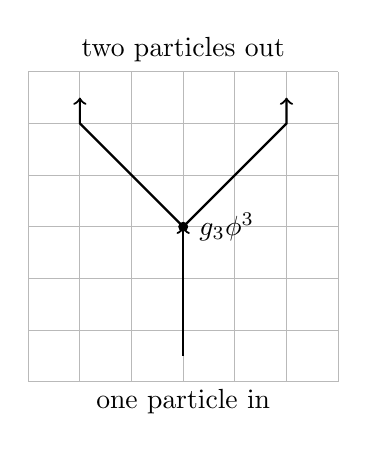
\begin{tikzpicture}[scale=0.82]
\draw[step=0.8,gray!55,thin] (0,0) grid (4.8,4.8);
\draw[thick,->] (2.4,0.4) -- (2.4,1.2) -- (2.4,2.0) -- (2.4,2.4);
\fill (2.4,2.4) circle (2.2pt);
\draw[thick,->] (2.4,2.4) -- (1.6,3.2) -- (0.8,4.0) -- (0.8,4.4);
\draw[thick,->] (2.4,2.4) -- (3.2,3.2) -- (4.0,4.0) -- (4.0,4.4);
\node[right] at (2.5,2.4) {$g_3\phi^3$};
\node at (2.4,-0.3) {one particle in};
\node at (2.4,5.15) {two particles out};
\end{tikzpicture}
\caption{이차 인자들은 입자가 삼차 분기 꼭짓점으로 들어오고 그곳에서 나가는 전파를 나타냅니다.}
\end{figure}

초기와 최종 상태에 입자가 하나씩 있는 진폭조차 더는 끊김 없는 단일 경로들의 합에 그치지 않습니다. 한 기여는 이차 도약들이 이어진 사슬을 통한 직접 전파입니다. 다른 기여에는 입자가 둘로 분리된 뒤 나중에 다시 합쳐지는 두 입방 인자가 들어 있습니다. 따라서 중간 상태에는 외부 상태보다 더 많은 입자가 있을 수 있습니다.\footnote{두 가지 경우는 01:09:44--01:11:36에 있는 도식으로부터 재구성됩니다.}

\begin{figure}[htbp]
\centering
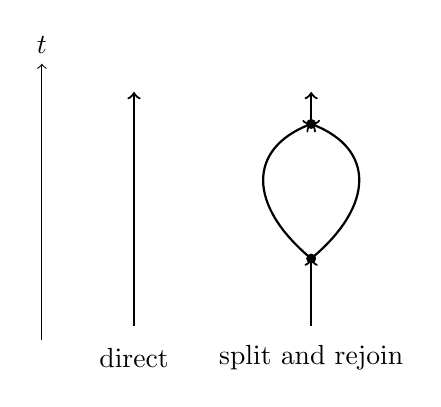
\begin{tikzpicture}[scale=0.9]
\draw[->] (-0.7,0) -- (-0.7,3.9) node[above] {$t$};
\draw[thick,->] (0.6,0.2) -- (0.6,3.5);
\node at (0.6,-0.25) {direct};
\draw[thick,->] (3.1,0.2) -- (3.1,1.15);
\fill (3.1,1.15) circle (2pt);
\draw[thick,->] (3.1,1.15) .. controls (2.2,1.9) and (2.2,2.7) .. (3.1,3.05);
\draw[thick,->] (3.1,1.15) .. controls (4.0,1.9) and (4.0,2.7) .. (3.1,3.05);
\fill (3.1,3.05) circle (2pt);
\draw[thick,->] (3.1,3.05) -- (3.1,3.5);
\node at (3.1,-0.25) {split and rejoin};
\end{tikzpicture}
\caption{같은 한 입자 진폭에 대한 직접 전파와 분기--재결합 기여.}
\end{figure}

전기역학에서 이에 해당하는 예는 전자가 광자를 방출한 뒤 나중에 다시 흡수하는 경우다. 이 방출과 재흡수의 이력은 전자가 한 점에서 다른 점으로 전파되는 진폭의 일부다. 고차에서는 방출과 흡수가 여러 번 일어난다. 광자가 전자--양전자 쌍으로 변환될 수 있으며, 그 중간 쌍을 이루는 전자와 양전자는 서로 광자를 교환할 수도 있다. 처음과 마지막의 입자 구성이 단순하다고 해서 중간 입자 구성까지 단순해야 하는 것은 아니다.\footnote{다음 재구성에 나오는 예들은 01:11:22--01:12:34에 있다.}

\begin{figure}[htbp]
\centering
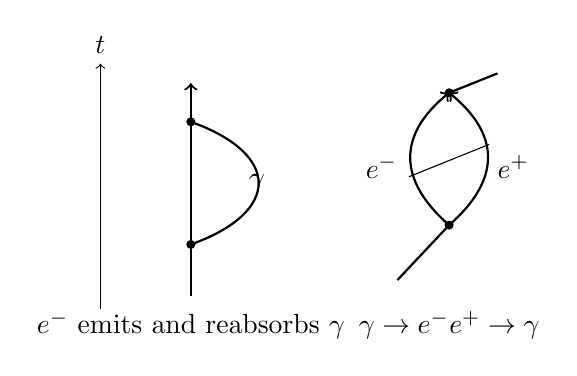
\begin{tikzpicture}[scale=0.82]
\draw[->] (-0.6,0) -- (-0.6,3.8) node[above] {$t$};
\draw[thick,->] (0.8,0.2) -- (0.8,3.5);
\fill (0.8,1.0) circle (2pt);
\fill (0.8,2.9) circle (2pt);
\draw[thick] (0.8,1.0) .. controls (2.2,1.5) and (2.2,2.4) .. (0.8,2.9);
\node[right] at (1.55,1.95) {$\gamma$};
\node at (0.8,-0.25) {$e^-$ emits and reabsorbs $\gamma$};
\draw[thick] (4.0,0.45) -- (4.8,1.3);
\fill (4.8,1.3) circle (2pt);
\draw[thick,->] (4.8,1.3) .. controls (4.0,2.0) and (4.0,2.7) .. (4.8,3.35);
\draw[thick,->] (4.8,1.3) .. controls (5.6,2.0) and (5.6,2.7) .. (4.8,3.35);
\fill (4.8,3.35) circle (2pt);
\draw[thick] (4.8,3.35) -- (5.55,3.65);
\draw[thin] (4.18,2.05) -- (5.42,2.55);
\node[left] at (4.15,2.2) {$e^-$};
\node[right] at (5.4,2.2) {$e^+$};
\node at (4.8,-0.25) {$\gamma\to e^-e^+\to\gamma$};
\end{tikzpicture}
\caption{전자의 자기 방출 기여와 전자--양전자 쌍이 포함된 광자 이력.}
\end{figure}

이러한 이력은 각각 지수함수 전개의 특정 항들의 곱에서 나온다. 그 계수에는 \(i\)의 적절한 거듭제곱, 지수급수에서 나오는 계승, 그리고 각 꼭짓점에 연결된 결합상수가 들어간다. 계수는 해당 이력의 기여를 정하지만, 지정된 초기 상태와 최종 상태에 대한 진폭은 같은 외부 상태를 갖는 모든 이력의 합이다.

\begin{classroomqa}
\lecturetimestamp{01:13:18}
\audiencequestion{같은 전체 과정이 여러 가지 서로 다른 이력으로 일어날 수 있고, 그 모든 이력이 진폭에 기여하나요?}
\lecturerresponse{그렇습니다. 과정의 진폭은 같은 초기 상태를 같은 최종 상태로 연결하는 서로 다른 모든 이력을 합해 구합니다.}
\end{classroomqa}

따라서 양자장론을 구성하는 데에는 서로 동등한 두 가지 방식이 있다. 장의 관점에서는 초기 장 배치와 최종 장 배치를 지정하고 그 사이의 모든 장 이력을 합한다. 입자의 관점에서는 장을 양자로 분해한다. 들어오는 입자 구성과 나가는 입자 구성을 지정하고, 이를 연결하는 모든 입자 이력을 합한다. 두 관점 모두 같은 라그랑지안으로 정해진다.

\section{사차항, 보존 법칙, 결합 상수}

4차 상호작용은 다음과 같다.
\begin{equation}
\mathcal{L}_{\mathrm{int}}=g_4\phi^4,
\end{equation}
한 점에서 장 인자 네 개를 갖는다. 국소적인 입자 해석에는 다음이 포함된다.
\begin{equation}
\begin{gathered}
2\longrightarrow2,
\qquad
1\longrightarrow3,
\qquad
3\longrightarrow1,\\
0\longrightarrow4,
\qquad
4\longrightarrow0.
\end{gathered}
\end{equation}
따라서 하나의 네 다리 꼭짓점은 두 입자 산란, 입자 하나가 셋으로 분열하는 과정, 셋이 하나로 합쳐지는 과정, 또는 네 다리가 모두 바깥쪽이나 안쪽을 향하는 과정을 나타낼 수 있다.\footnote{방향은 01:14:28--01:15:18의 도표를 바탕으로 재구성한 것이다.}

\begin{figure}[htbp]
\centering
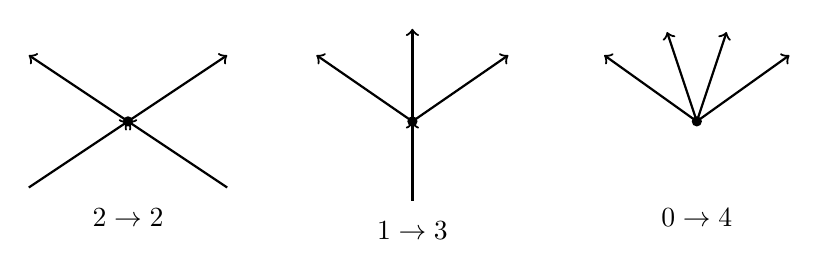
\begin{tikzpicture}[scale=0.84]
\fill (0,0) circle (2.2pt);
\draw[thick,->] (-1.5,-1.0) -- (0,0);
\draw[thick,->] (1.5,-1.0) -- (0,0);
\draw[thick,->] (0,0) -- (-1.5,1.0);
\draw[thick,->] (0,0) -- (1.5,1.0);
\node at (0,-1.45) {$2\to2$};
\begin{scope}[xshift=4.3cm]
\fill (0,0) circle (2.2pt);
\draw[thick,->] (0,-1.2) -- (0,0);
\draw[thick,->] (0,0) -- (-1.45,1.0);
\draw[thick,->] (0,0) -- (0,1.4);
\draw[thick,->] (0,0) -- (1.45,1.0);
\node at (0,-1.65) {$1\to3$};
\end{scope}
\begin{scope}[xshift=8.6cm]
\fill (0,0) circle (2.2pt);
\draw[thick,->] (0,0) -- (-1.4,1.0);
\draw[thick,->] (0,0) -- (-0.45,1.35);
\draw[thick,->] (0,0) -- (0.45,1.35);
\draw[thick,->] (0,0) -- (1.4,1.0);
\node at (0,-1.45) {$0\to4$};
\end{scope}
\end{tikzpicture}
\caption{4개 다리 상호작용 꼭짓점의 세 가지 국소적 방향 배치.}
\end{figure}

국소 해석 \(0\to4\)만으로 진공에서 입자 네 개가 물리적 과정으로 나타날 수 있다는 뜻은 아니다. 꼭짓점은 가능한 모든 시공간 위치에 대해 여전히 합산해야 한다. 제안된 외부 상태에서 에너지를 보존할 수 없다면, 각 위치에서 오는 위상들이 상쇄된다.

\begin{classroomqa}
\lecturetimestamp{01:15:18}
\audiencequestion{네 다리가 모두 바깥을 향한 배치는 최종 상태에 입자 네 개가 저절로 나타나는 과정을 뜻하나요?}
\lecturerresponse{이는 4장 연산자를 국소적으로 해석한 한 가지 방식이지만, 들어오는 에너지가 없는 과정은 에너지 보존에 어긋납니다. 가능한 모든 시공간 위치의 꼭짓점에서 오는 진폭을 더하면 서로 상쇄되어 0이 됩니다.}
\end{classroomqa}

\begin{classroomqa}
\lecturetimestamp{01:15:58}
\audiencequestion{에너지 보존과 운동량 보존은 계산 자체에서 나오는 것인가요?}
\lecturerresponse{그렇습니다. 꼭짓점을 모든 시간에 대해 적분하면 에너지 보존이 성립하고, 모든 공간에 대해 적분하면 운동량 보존이 성립합니다. 꼭짓점 위치에 대한 합은 에너지와 운동량이 모두 보존되지 않으면 사라집니다.}
\end{classroomqa}

이러한 보존 법칙을 만족하는 한, 라그랑지안이 허용하는 모든 그래프는 어떤 진폭에 기여합니다. 그 기여의 크기는 부분적으로 각 상호작용 항의 계수에 따라 달라집니다. 입방항과 사차항의 계수를 \(G_3\) 및 \(G_4\)로 씁시다. 세 다리 꼭짓점마다 \(G_3\) 인자 하나가 기여하고, 네 다리 꼭짓점마다 \(G_4\) 인자 하나가 기여합니다. 따라서 입방 꼭짓점이 \(V_3\)개이고 사차 꼭짓점이 \(V_4\)개인 그래프의 결합 상수 의존성은 도식적으로 다음과 같습니다.
\begin{equation}
\mathcal{A}_{\mathrm{graph}}
\propto G_3^{V_3}G_4^{V_4}.
\end{equation}

이 결합상수들이 작으면 꼭짓점이 적은 그래프가 일반적으로 많은 그래프보다 크게 기여한다. 꼭짓점이 하나 추가될 때마다 작은 인자가 하나 더 붙는다. 덕분에 섭동 합이 유용할 가능성이 생긴다. 가장 단순한 그래프에서 시작해 점차 작은 보정을 차례로 더하면 된다.

완전한 급수가 실제로 수렴하는지는 어려운 문제다. 결합상수가 작으면 항들의 크기 순서가 그럴듯해지지만, 그것만으로 모든 수렴 문제에 답할 수는 없다. 결합상수가 크면 순진한 급수는 아예 실패할 수 있다. 그렇다고 기초 이론이 틀렸다는 뜻은 아니다. 결합상수의 거듭제곱으로 전개하는 방식이 계산에 적절하지 않았다는 뜻일 수 있다. 여기서 논의하는 방법은 결합상수가 충분히 작아 꼭짓점 네 개짜리 그래프가 꼭짓점 두 개짜리 그래프보다 훨씬 작을 때 가장 직접적으로 유용하다.

\begin{classroomqa}
\lecturetimestamp{01:19:24}
\audiencequestion{색 이론도 같은 방식으로 다룰 수 있나요?}
\lecturerresponse{그렇습니다. 색 이론도 같은 방식으로 정식화할 수 있으며, 뒤에서 다룰 것입니다.}
\end{classroomqa}

\section{전파자, 꼭짓점, 그리고 상호보완적인 관점}

다음 과제는 입자를 열거하고 라그랑지안이나 파인만 규칙으로 그 동역학을 표현하는 것이다. 두 방식은 같은 정보를 서로 다르게 나타낸다. 2차 항은 한 점에서 다른 점으로의 전파를 나타낸다. 그 전파를 나타내는 선을 전파자라고 한다. 장이 세 개 이상 포함된 항은 선들이 만나는 지점을 나타낸다. 그 만나는 점이 꼭짓점이다. 예를 들면 다음과 같다.
\begin{equation}
\begin{aligned}
\text{quadratic term}
&\longleftrightarrow \text{propagator},\\
G_3\phi^3
&\longleftrightarrow \text{three-leg vertex}.
\end{aligned}
\end{equation}

입자마다 양자장을 하나씩 지정하고, 각 입자의 질량과 상호작용을 모두 포함하는 라그랑지안 하나를 쓰면 이론을 규정할 수 있다. 또는 모든 전파자와 허용된 꼭짓점, 그리고 각 꼭짓점에 붙는 계수를 열거해도 된다. 어느 쪽 목록이든 어떤 과정이 가능한지, 그 과정의 그래프에 진폭을 어떻게 부여하는지 알려 준다.

예를 들어 전자 두 개는 광자를 교환하며 산란할 수 있다. 각 전자 선에는 전자--전자--광자 꼭짓점이 있고, 광자 전파자가 두 꼭짓점을 잇는다.\footnote{이 도표는 01:21:38의 예를 바탕으로 재구성한 것이다.}

\begin{figure}[htbp]
\centering
\begin{tikzpicture}[scale=0.95]
\draw[->] (-0.6,-0.2) -- (0.2,1.4);
\draw[->] (0.2,1.4) -- (-0.7,3.1);
\draw[->] (3.5,-0.2) -- (2.7,1.4);
\draw[->] (2.7,1.4) -- (3.6,3.1);
\fill (0.2,1.4) circle (2pt);
\fill (2.7,1.4) circle (2pt);
\draw[thick] (0.2,1.4) -- (2.7,1.4);
\node[above] at (1.45,1.4) {$\gamma$};
\node[left] at (-0.2,0.5) {$e^-$};
\node[right] at (3.1,0.5) {$e^-$};
\end{tikzpicture}
\caption{광자 교환으로 일어나는 전자 두 개의 산란.}
\end{figure}

라그랑지안은 이 그래프의 진폭을 정하고 이를 제한하는 대칭성과 보존 법칙을 담고 있다. 시간 방향을 나타내는 그림에서는 아래쪽에 놓인 입자들이 초기 배치를 이루고 위쪽에 놓인 입자들이 최종 배치를 이룬다.

\begin{classroomqa}
\lecturetimestamp{01:22:06}
\audiencequestion{파인만 도표에서 아래쪽 입자들이 초기 배치이고 위쪽 입자들이 최종 배치인가요?}
\lecturerresponse{그렇습니다. 아래쪽은 초기 입자 배치이고 위쪽은 최종 입자 배치입니다.}
\end{classroomqa}

입자 관점과 장 관점은 보통의 양자역학에서 운동량과 위치가 상호보완적인 기술인 것처럼 서로 보완적이다. 이들은 서로 다른 기저에서 같은 계를 기술한다. 이에 대응하는 불확정성도 있다. 입자 수를 정확히 지정하면 장의 값은 불확정하고, 장의 값을 정확히 지정하면 입자 수는 불확정하다. 어느 한 관점이 다른 관점을 대체하지 않으며, 라그랑지안은 두 관점 모두에서 유용하다.

\begin{classroomqa}
\lecturetimestamp{01:23:26}
\audiencequestion{결합상수는 이론이 예측하나요, 아니면 실험으로 정하나요?}
\lecturerresponse{대칭성이 때로는 한 결합상수를 다른 결합상수와 연관 지을 수 있지만, 그 수치는 대체로 실험으로 정합니다.}
\end{classroomqa}

\section{실험으로 정하는 입력값과 폭넓은 예측}

양자장론 자체에는 우아함과 아름다움이 있다. 그러나 사실들을 열거하기 시작하면---어떤 입자가 있는지, 질량은 얼마인지, 결합상수는 얼마인지---목록은 엉망이다. 대칭성이 제공하는 일관성을 빼면 거의 일관성이 없는, 매우 볼품없는 난잡한 목록이다. 대칭성은 서로 다른 종류의 입자와 그 과정들을 연관 짓지만, 그 범위에는 한계가 있다. 목록의 상당 부분은 동기가 뚜렷하지 않은 여러 종류의 입자에 관한, 서로 비교적 무관한 사실들의 큰 집합으로 남아 있다.

\begin{classroomqa}
\lecturetimestamp{01:24:58}
\audiencequestion{실험으로 측정한 결합상수를 왜 그토록 확신할 수 있나요?}
\lecturerresponse{결합상수를 측정한 뒤 그 값을 바꾸면 예측이 틀립니다. 그 값을 사용하는 여러 계산을 통해 타당성이 검증됩니다.}
\end{classroomqa}

입자가 너무 많다는 것은 장도 너무 많다는 뜻이다---미적 감각으로 받아들이기에는 지나치게 많다. 대략 백 개 남짓이다. 결합상수도 많고, 대체로 실험에서 얻은 숫자들이며, 질량도 많아서 그 값의 범위가 매우 넓다. 그 사이에 관계가 몇 가지 있기는 하지만, 극히 일부에 불과하다.

그러나 일단 그 값들을 알면 계산을 시작할 수 있다. 그 값들을 알면 그걸로 충분하다. 그 입자에 관한 것은 무엇이든 매우 정밀하게 계산할 수 있다. 쿼크, 전자, 광자 등을 다루는 내용은 원자물리학, 입자물리학, 핵물리학, 화학, 어쩌면 생물학까지 이어진다. 입력값의 양은 바라는 것보다 많을 수 있지만, 그로부터 얻는 결과는 방대하다.

\section{섭동 전개의 예로 보는 양자전기역학}

양자전기역학은 결합상수 전개의 구체적인 예를 제공한다.

\begin{classroomqa}
\lecturetimestamp{01:26:12}
\audiencequestion{전자와 광자의 경우, \(G_n\) 유형의 상호작용 결합상수는 몇 개나 있나요?}
\lecturerresponse{기본 상호작용 결합상수는 하나, 전하 \(e\)입니다. 전자가 들어오고 나가며 광자가 방출되거나 흡수되는 꼭짓점에 붙는 \(G_3\) 유형의 계수입니다.}
\end{classroomqa}

스피너 행렬과 지표를 생략하면 상호작용의 장 구성은 개략적으로 다음과 같다.
\begin{equation}
\mathcal{L}_{\mathrm{QED,int}}
\sim e\,(\text{electron bilinear})\,A,
\end{equation}
여기서 \(A\)는 광자 장을 나타낸다. 자세한 디랙 행렬 구조는 계수를 세는 논의에 필요하지 않다. 기본적인 양자전기역학 규칙은 전자가 광자를 방출하거나 흡수하는 것이다. 더 복잡한 양자전기역학 그래프는 모두 이 하나의 꼭짓점을 반복해서 사용해 구성된다.\footnote{개략적인 꼭짓점은 01:26:42에서 재구성했다. 원문에서는 자세한 행렬 구조를 의도적으로 생략한다.}

\begin{figure}[htbp]
\centering
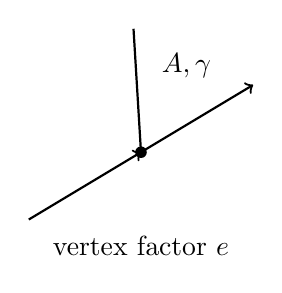
\begin{tikzpicture}[scale=0.95]
\draw[thick,->] (-1.5,-0.9) -- (0,0);
\draw[thick,->] (0,0) -- (1.5,0.9);
\draw[thick] (0,0) -- (-0.1,1.65);
\fill (0,0) circle (2.2pt);
\node[right] at (0.15,1.15) {$A,\gamma$};
\node at (0,-1.25) {vertex factor $e$};
\end{tikzpicture}
\caption{양자전기역학의 기본 전자--전자--광자 꼭짓점.}
\end{figure}

\begin{classroomqa}
\lecturetimestamp{01:27:38}
\audiencequestion{전자--양성자 산란은 어떤가요?}
\lecturerresponse{기본적인 원자 모형에서는 양성자를 고정된 무한히 무거운 점 전하원---즉 제자리에 못 박아 둔 무거운 입자로 이상화할 수 있습니다. 양성자 자체의 양자장 동역학은 양성자와 중성자의 내부 이론을 포함할 때에만 다룹니다.}
\end{classroomqa}

\begin{classroomqa}
\lecturetimestamp{01:28:30}
\audiencequestion{전자는 그 양성자에 대해 빛의 속도에 가깝게 움직일 수 있나요?}
\lecturerresponse{그렇습니다.}
\end{classroomqa}

전자에 의한 광자 산란을 생각해 보자. 최저 차수 그래프에는 전자--전자--광자 꼭짓점이 두 개 있다. 따라서 진폭은 \(e^2\)에 비례한다.
\begin{equation}
\mathcal{A}_{\mathrm{lowest}}\propto e^2.
\end{equation}
확률, 또는 이에 동등하게 결합상수에 대한 단면의 의존성은 절댓값의 제곱으로 주어지므로 \(e^4\)에 비례한다.
\begin{equation}
P_{\mathrm{lowest}}\ \text{or}\ \sigma_{\mathrm{lowest}}
\propto e^4.
\end{equation}
통상적인 무차원 정규화에서 전하 결합상수는 작다. 따라서 실제 산란이 일어날 가능성은 광자가 산란 없이 그냥 지나갈 가능성보다 훨씬 낮다.

이 차수에는 이미 그래프가 두 개 있다. 한 시간 순서에서는 들어오는 광자를 흡수한 뒤 나중에 나가는 광자를 방출한다. 다른 순서에서는 들어오는 광자를 흡수하기 전에 나가는 광자를 방출한다. 두 진폭 모두 기여한다.\footnote{두 시간 순서는 01:28:42와 01:30:18의 도표를 바탕으로 재구성했다.}

\begin{figure}[htbp]
\centering
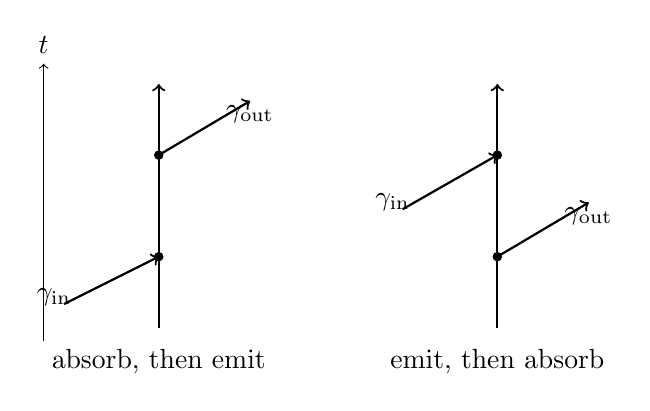
\begin{tikzpicture}[scale=0.86]
\draw[->] (-0.7,0) -- (-0.7,4.1) node[above] {$t$};
\draw[thick,->] (1.0,0.2) -- (1.0,3.8);
\fill (1.0,1.25) circle (2pt);
\fill (1.0,2.75) circle (2pt);
\draw[thick,->] (-0.4,0.55) -- (1.0,1.25);
\draw[thick,->] (1.0,2.75) -- (2.35,3.55);
\node[left] at (-0.15,0.65) {$\gamma_{\mathrm{in}}$};
\node[right] at (1.85,3.35) {$\gamma_{\mathrm{out}}$};
\node at (1.0,-0.3) {absorb, then emit};
\begin{scope}[xshift=5.0cm]
\draw[thick,->] (1.0,0.2) -- (1.0,3.8);
\fill (1.0,1.25) circle (2pt);
\fill (1.0,2.75) circle (2pt);
\draw[thick,->] (1.0,1.25) -- (2.35,2.05);
\draw[thick,->] (-0.4,1.95) -- (1.0,2.75);
\node[right] at (1.85,1.85) {$\gamma_{\mathrm{out}}$};
\node[left] at (-0.15,2.05) {$\gamma_{\mathrm{in}}$};
\node at (1.0,-0.3) {emit, then absorb};
\end{scope}
\end{tikzpicture}
\caption{전자--광자 산란의 최저 차수 시간 순서 두 가지.}
\end{figure}

따라서 최저 차수 진폭은 그래프 하나의 진폭이 아니라 두 진폭의 합이다.
\begin{equation}
\begin{aligned}
\mathcal{A}^{(2)}
&=
\mathcal{A}_{\mathrm{absorb\ then\ emit}}
+\mathcal{A}_{\mathrm{emit\ then\ absorb}},\\
\mathcal{A}^{(2)}&\propto e^2.
\end{aligned}
\end{equation}

고차 보정에는 기본 꼭짓점이 더 추가된다. 전자 선에 내부 광자를 하나 더 연결하면 \(e\) 인자가 두 개 더 붙어, 진폭에는 \(e^4\)에 비례하는 기여가, 그 절댓값을 제곱한 값에는 \(e^8\)에 비례하는 기여가 생긴다. 광자 선에 전자--양전자 삽입이 들어갈 수도 있으며, 이 경우에도 기본 꼭짓점과 추가적인 \(e\) 거듭제곱이 더해진다. 이는 예시일 뿐 전부는 아니다. 추가 광자는 여러 위치에 연결할 수 있다.\footnote{고차 구조는 01:30:38--01:31:16에서 재구성했다.}

\begin{figure}[htbp]
\centering
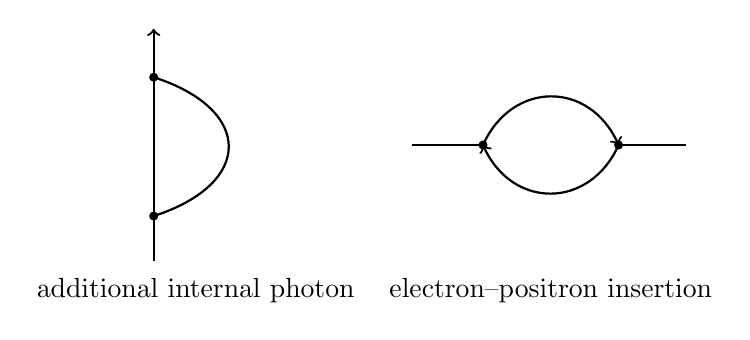
\begin{tikzpicture}[scale=0.82]
\draw[thick,->] (0.9,0.2) -- (0.9,3.8);
\fill (0.9,0.9) circle (2pt);
\fill (0.9,3.05) circle (2pt);
\draw[thick] (0.9,0.9) .. controls (2.45,1.4) and (2.45,2.55) .. (0.9,3.05);
\node at (1.55,-0.25) {additional internal photon};
\begin{scope}[xshift=5.1cm]
\draw[thick] (-0.2,2.0) -- (0.9,2.0);
\fill (0.9,2.0) circle (2pt);
\fill (3.0,2.0) circle (2pt);
\draw[thick,->] (0.9,2.0) .. controls (1.35,3.0) and (2.55,3.0) .. (3.0,2.0);
\draw[thick,->] (3.0,2.0) .. controls (2.55,1.0) and (1.35,1.0) .. (0.9,2.0);
\draw[thick] (3.0,2.0) -- (4.05,2.0);
\node at (1.95,-0.25) {electron--positron insertion};
\end{scope}
\end{tikzpicture}
\caption{기본 꼭짓점을 추가하고 \(e\)의 더 높은 거듭제곱을 더하는 고차 양자전기역학 구조 두 가지.}
\end{figure}

따라서 양자전기역학 전개는 \(e^2\)의 연속된 거듭제곱으로 진행된다. 비슷한 복잡성을 지닌 구조가 하나 추가될 때마다 진폭에 전하의 거듭제곱이 두 번 더해진다. 여기서 사용하는 정규화에서는 이러한 보정이 앞선 차수보다 진폭 기준으로 대략 백 배에서 이백 배 정도 작다. 더 복잡한 그래프일수록 기여가 점차 작아지므로 섭동 합이 유용할 가능성이 생긴다.

확률은 각 그래프의 진폭을 따로 제곱한 뒤 그 제곱들을 더해서 구하지 않는다. 먼저 같은 외부 과정을 나타내는 모든 진폭을 더한다.
\begin{equation}
\mathcal{A}_{\mathrm{total}}=\sum_r\mathcal{A}_r.
\end{equation}
그런 다음에야 다음을 계산한다.
\begin{equation}
P=\left|\mathcal{A}_{\mathrm{total}}\right|^2
=\left|\sum_r\mathcal{A}_r\right|^2.
\end{equation}
서로 다른 그래프 사이의 교차항은 간섭항이다. 규칙은 간단하고 중요하다. 먼저 더한 다음 제곱한다.

\section{입자 목록과 표준 모형을 향하여}

전파자, 꼭짓점, 결합상수 계산, 간섭까지 갖추었으니 이제 본격적으로 입자물리학을 기술할 수 있다. 입자의 이름을 정하고 질량을 지정하며, 이론과 실험을 통해 일부씩 정해지는 라그랑지안을 쓰고, 그 라그랑지안에서 대칭성을 직접 살펴볼 수 있다. 같은 틀에서 표준 모형과 그 성질도 다룰 수 있다.

\begin{classroomqa}
\lecturetimestamp{01:33:22}
\audiencequestion{일정한 질량 계수 \(m^2\)를 힉스 장으로 대체할 수 있나요?}
\lecturerresponse{그렇습니다. 바로 그 생각이 맞으며, 그 메커니즘은 뒤에서 다룰 것입니다.}
\end{classroomqa}

\begin{classroomqa}
\lecturetimestamp{01:33:42}
\audiencequestion{이웃한 격자점 \(x\)와 \(x'\)가 서로 다른 시간에 있을 수 있나요?}
\lecturerresponse{그렇습니다. 시간 방향의 이웃점일 수 있습니다. 이것이 격자에서 수직 방향 전파를 나타내는 방식입니다.}
\end{classroomqa}

이웃한 점들에서는 유한 차분의 제곱에 같은 위치 항과 교차 링크 항이 모두 들어간다.
\begin{equation}
\bigl[\phi(x)-\phi(x')\bigr]^2
=
\phi(x)^2+\phi(x')^2-2\phi(x)\phi(x').
\end{equation}

\begin{classroomqa}
\lecturetimestamp{01:33:56}
\audiencequestion{입자가 그 자리에 가만히 있는 것을 나타내는 항은 무엇인가요?}
\lecturerresponse{유한 차분의 제곱에 있는 같은 위치 항 \(\phi(x)^2\)와 \(\phi(x')^2\)는 가만히 있는 경우를 나타내고, 교차 항 \(\phi(x)\phi(x')\)는 움직이는 해석을 제공한다. 명시적인 질량 항도 같은 위치에서 가만히 있는 인자를 더한다.}
\end{classroomqa}
